%-shell-escape, якщо використовуєте minted
\documentclass[a4paper, 12pt, oneside]{extarticle}
\input{$HOME/Templates/lpnu_doc_templates/settings/preamble.tex}
% якщо домахуються за Times New Roman, то
% використовуєте xelatex і цей файл:
\input{$HOME/Templates/lpnu_doc_templates/settings/font_styles.tex}
\input{$HOME/Templates/lpnu_doc_templates/settings/minted_settings.tex}

\newcommand\Variant{4}
\newcommand\Date{22.04.\the\year}
\newcommand\Discipline{Об'єктно-орієнтоване програмування}
\newcommand\Instructor{Патерега Ю. І.}

\newcommand\Type{\Lab}
\newcommand\Number{5}
\newcommand\Topic{Інкапсуляція. Наслідування. Поліморфізм. Віртуальні функції}

\setcounter{secnumdepth}{0}

\begin{document}
\Margins

\Margins
%\begin{wrapfigure}[3]{l}{.27\textwidth}
%\includegraphics[width=.28\textwidth]{$UNI/.templates/lpnu_logo.png}
%\end{wrapfigure}

%\noindent\textbf{Прізвище:} \Lname \\
%\noindent\textbf{Ім'я:} \Fname \\
%\noindent\textbf{Група:} \Group \\
%\noindent\textbf{Варіант:} \Variant \\
%\noindent\textbf{Дата захисту:} \Date \\
%\\
%\noindent\textbf{Кафедра:} \Department \\
%\noindent\textbf{Дисципліна:} \Discipline \\
%\noindent\textbf{Перевірив:} \Instructor \\

%%\medskip\bigskip

%\begin{center}
%	\textbf{ЗВІТ}		\\
%	до \Type~\No\Number	\\
%	на тему ``\Topic''	\\
%\end{center}

% \begin{table}
%   \begin{tabularx}{\textwidth}{|c|X|X|}
%     \hline
%     % Image & Content & Additional Info \\
%     % \hline
% 	  \multirow{3}{*}{\includegraphics[width=4cm]{$UNI/.templates/lpnu_logo.png}}
% 	  & \textbf{ЗВО:}
% 	  Національний університет ``Львівська Політехніка''.
% 	  & \textbf{Тема:}
% 	  \Topic
% 	  \\
% 	  & \textbf{Навчальний рік:}
% 	  2023/2024
% 	  & \textbf{Інститут}
% 	  комп'ютерних наук та інформаційних технологій
% 	  \\
% 	  & \textbf{Семестр:}
% 	  осінній
% 	  & \textbf{Група:}
% 	  \Group
% 	  \\
% 	  & \textbf{Навчальна дисципліна:}
% 	  \Discipline
% 	  & \textbf{Студент:}
% 	  Мілюхін Олександр
% 	  \\
% 	  & \textbf{Кафедра}
% 	  систем автоматизованого проектування
% 	  &
% 	  \\
% 	  & \textbf{Викладач:}
% 	  Чумакевич В. В.
% 	  &
% 	  \\
%     \hline
%   \end{tabularx}
% \end{table}

\setlength{\textfloatsep}{-16pt}
% \setlength{\intextsep}{0pt}

\begin{table}
	\begin{tabular}{|l|l|p{6cm}|}
    \hline
    % Image & Content & Additional Info \\
    % \hline
	  \makecell[l]{
	  \includegraphics[width=3.37cm]{$UNI/.templates/lpnu_logo.png}
  }
	  & \makecell[l]{
	  \textbf{ЗВО:}
	  Національний університет \\ ``Львівська Політехніка''.
	  \\
	  \textbf{Навчальний рік:}
	  2023/2024
	  \\
	  \textbf{Семестр:}
	  осінній
	  \\
	  \textbf{Навчальна дисципліна:} \\
	  \Discipline
	  \\
	  \textbf{Кафедра}
	  систем автоматизованого \\ проектування
	  \\
	  \textbf{Викладач:}
	  Чумакевич В. В.
}
	  & \makecell [l] {
	  \textbf{Тема:}
	  \Topic
	  \\
          \textbf{Інститут}
	  комп'ютерних наук та \\ інформаційних технологій
	  \\
	  \textbf{Група:}
	  \Group
	  \\
	  \textbf{Студент:}
	  Мілюхін Олександр
  }
  \\
    \hline
  \end{tabular}
\end{table}
\section{Мета роботи}

% \begin{table}
%   \begin{tabularx}{\textwidth}{|p{6cm}|c|c|}
% 	  \hline
%     \multirow{3}{*}{\includegraphics[width=6cm]{$UNI/.templates/lpnu_logo.png}}
% 	  & ЗВО: Національний університет ``Львівська Політехніка''
% 	  & Additional Info 1 \\
%     & Content 2 & Additional Info 2 \\
%     & Content 3 & Additional Info 3 \\
% 	  \hline
%   \end{tabularx}
% \end{table}

% \begin{table}
%   \begin{tabular}{|c|c|c|}
%     \hline
%     \multirow{3}{*}{\includegraphics[width=3cm]{$UNI/.templates/lpnu_logo.png}} & \makecell{Content 1 \\ Content 2 \\ Content 3} & \makecell{Additional Info 1 \\ Additional Info 2 \\ Additional Info 3} \\
%     \hline
%   \end{tabular}
% \end{table}


Ознайомитись з основними принципами наслідування властивостей
об’єктів
та
навчитись
створювати
похідні
класи.
Освоїти
поняттям
поліморфізму та методами реалізації поліморфізму в мові програмування С++.

\section*{Індивідуальне завдання}

\subsection*{Завдання 1}

Необхідно побудувати ієрархію класів відповідно схемі наслідування,
наведеній у варіанті завдання.
Кожен клас повинен містити конструктор
ініціалізації, і функцію show для виведення значень.
Функція main повинна
ілюструвати ієрархію наслідування.

\begin{figure}[h]
	\centering
	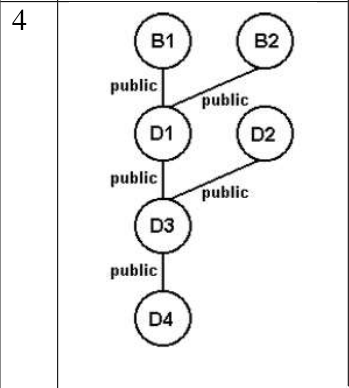
\includegraphics[width=.3\textwidth]{/home/sasha/Documents/uni/2-сем/OOP/labs/lab-5/pic-selected-230411-1039-16.png}
	\caption{діаграма до завдання 1}
\end{figure}

\subsection*{Завдання 2}

Створити клас для *зберігання бази даних*, вказаної у таблиці з
відповідними полями.

\section*{Етапи розв'язку}

\subsection*{Завдання 1}
Проаналізував діаграму, написав чорнову ієрархію в заголовному файлі.
Далі реалізовував та виправляв помилки.

\subsection*{Завдання 2}

Реалізував клас Ware, на його базі --- SweetRoll.
Була проблема зі збереженням поля класу типу string
у файлі, тому я дослідив цю тему й вирішив
реалізувати збереження за допомогою бібліотеки cereal.
Створив шаблон для запису як об'єкта класу Ware, так і об'єкта класу SweetRoll

\section*{Коди програм}

\subsection*{Код програми (завдання 1)}

\subsubsection{hier.h}
\inputminted{c++}{task1/include/hier.h}
\subsubsection{hier.cpp}
\inputminted{c++}{task1/src/hier.cpp}
\subsubsection{main.cpp}
\inputminted{c++}{task1/src/main.cpp}

\subsection*{Результат виконання програми}

\begin{verbatim}
[sasha@honeypot ~uni/OOP/labs/lab-5/task1/src]$ ./main
D1
B1 constructor
B2 constructor
D1 constructor
222
D1 destructor
B2 destructor
B1 destructor
D2
D2 constructor
50
D3
B1 constructor
B2 constructor
D1 constructor
D2 constructor
D3 constructor
63
D4
B1 constructor
B2 constructor
D1 constructor
D2 constructor
D3 constructor
D4 constructor
63
D4 destructor
D3 destructor
D2 destructor
D1 destructor
B2 destructor
B1 destructor
D3 destructor
D2 destructor
D1 destructor
B2 destructor
B1 destructor
D2 destructor
D1 destructor
B2 destructor
B1 destructor
\end{verbatim}

\subsection*{Код програми (завдання 2)}

\subsubsection{ware.h}
\inputminted{c++}{task2/include/ware.h}
\subsubsection{object_store.h}
\inputminted{c++}{task2/include/object_store.h}
\subsubsection{sweet_roll.h}
\inputminted{c++}{task2/include/sweet_roll.h}

\subsubsection{ware.cpp}
\inputminted{c++}{task2/src/ware.cpp}
\subsubsection{sweet_roll.cpp}
\inputminted{c++}{task2/src/sweet_roll.cpp}
\subsubsection{main.cpp}
\inputminted{c++}{task2/src/main.cpp}

\subsection*{Результат виконання програми}

\verbatiminput{out}

\section*{Висновок}

Виконавши цю лабораторну роботу, я закріпив свої
знання успадкування в c++ та вміння його реалізовувати.

\section*{Відповіді на контрольні запитання}
\begin{itemize}
	\question У чому суть наслідування в ООП?
	\answer У скороченні коду шляхом створення об'єктів, чиїх
		властивостей далі можуть набути інші.
	\question Який загальний синтаксис опису похідного класу?
	\answer class клас_нащадок : <мод доступу> батьківський_клас

	\question Який тип доступу буде мати поле зі специфікатором public при захищеному наслідуванні?
	\answer protected

	\question Який порядок виклику конструкторів та деструкторів при наслідуванні?
		\answer \begin{enumerate}
				\item конструктор базового класу
				\item конструктор похідного класу
				\item деструктор похідного класу
				\item деструктор базового класу
			\end{enumerate}
	\question У чому суть поліморфізму в ООП?
	\answer у підвищенні гнучкості коду завдяки створенню різних
		об'єктів з однаковими методами, що в кожному мають іншу
		реалізацію.
	\question Що таке віртуальна функція?
	\answer Віртуальна функція - це метод класу, який може бути перевизначений в похідних класах.
	\question Яким чином здійснюється динамічна ідентифікація типів?
	\answer За допомогою механізму RTTI (Run-Time Type Identification) - ідентифікації типів відповідно до виконання програми.

Механізм RTTI дозволяє дізнатись тип об'єкта в рантаймі, тобто під час виконання програми. Для цього в C++ використовується оператор dynamic_cast, який дозволяє перевірити, чи можна привести певний об'єкт до певного типу.
	\question В яких випадках деструктор має бути віртуальним?
	\answer Деструктор класу має бути віртуальним, якщо клас має хоча б одну віртуальну функцію і використовується як базовий клас. Інакше
		під час знищення об'єкта-нащадка може не статися його виклик.


\end{itemize}

\end{document}
